%%%%%%%%%%%%%%%%%%%%%%%%%%%%%%%%%%%%%%%%%%%%%%%%%%%%%%%%%%%%%%%%%%%%%%%%%%%%%%%%%
% Template: Article
%
% Por: Abrantes Araújo Silva Filho
%      abrantesasf@gmail.com
%
% Citação: Se você gostou deste template, por favor ajude a divulgá-lo mantendo
%          o link para meu repositório GitHub em:
%          https://github.com/abrantesasf/LaTeX
%%%%%%%%%%%%%%%%%%%%%%%%%%%%%%%%%%%%%%%%%%%%%%%%%%%%%%%%%%%%%%%%%%%%%%%%%%%%%%%%%




%%%%%%%%%%%%%%%%%%%%%%%%%%%%%%%%%%%%%%%%%%%%%%%%%%%%%%%%%%%%%%%%%%%%%%%%%%%%%%%%%
%%% Configura o tipo de documento, papel, tamanho da fonte e informações básicas
%%% para as proriedades do PDF/DVIPS e outras propriedades do documento
\RequirePackage{ifpdf}
\ifpdf
  % Classe, língua e tamanho da fonte padrão. Outras opções a considerar:
  %   draft
  %   onecolumn (padrão) ou twocolumn (OU usar o package multicol)
  %   fleqn com ou sem leqno (alinhamento à esquerda das fórmulas e dos números)
  %   oneside (padrão para article ou report) ou twoside (padrão para book)
  \documentclass[pdftex, brazil, 12pt, twoside]{article}
\else
  % Classe, língua e tamanho da fonte padrão. Outras opções a considerar:
  %   draft
  %   onecolumn (padrão) ou twocolumn (OU usar o package multicol)
  %   fleqn com ou sem leqno (alinhamento à esquerda das fórmulas e dos números)
  %   oneside (padrão para article ou report) ou twoside (padrão para book)
  \documentclass[brazil, 12pt]{article}
\fi


%%%%%%%%%%%%%%%%%%%%%%%%%%%%%%%%%%%%%%%%%%%%%%%%%%%%%%%%%%%%%%%%%%%%%%%%%%%%%%%%%
%%% Carrega pacotes iniciais necessários para estrutura de controle e para a
%%% criação e o parse de novos comandos
\usepackage{ifthen}
\usepackage{xparse}


%%%%%%%%%%%%%%%%%%%%%%%%%%%%%%%%%%%%%%%%%%%%%%%%%%%%%%%%%%%%%%%%%%%%%%%%%%%%%%%%%
%%% Configuração do tamanho da página, margens, espaçamento entrelinhas e, se
%%% necessário, ativa a indentação dos primeiros parágrafos.
\ifpdf
  \usepackage[pdftex]{geometry}
\else
  \usepackage[dvips]{geometry}
\fi
\geometry{a4paper, left=2.6cm, right=4.0cm, top=3.0cm, bottom=3.4cm}

\usepackage{setspace}
  \singlespacing
  %\onehalfspacing
  %\doublespacing


%%%%%%%%%%%%%%%%%%%%%%%%%%%%%%%%%%%%%%%%%%%%%%%%%%%%%%%%%%%%%%%%%%%%%%%%%%%%%%%%%
%%% Configurações de cabeçalho e rodapé:
\usepackage{fancyhdr}
\setlength{\headheight}{1cm}
\setlength{\footskip}{1.5cm}
\renewcommand{\headrulewidth}{0.3pt}
\renewcommand{\footrulewidth}{0.0pt}
\pagestyle{fancy}
\renewcommand{\sectionmark}[1]{%
  \markboth{\uppercase{#1}}{}}
\renewcommand{\subsectionmark}[1]{%
  \markright{\uppercase{\thesubsection \hspace{0.1cm} #1}}{}}
\fancyhead{}
\fancyfoot{}
\newcommand{\diminuifonte}{%
    \fontsize{9pt}{9}\selectfont
}
\newcommand{\aumentafonte}{%
    \fontsize{12}{12}\selectfont
}
% Configura cabeçalho e rodapé para documentos TWOSIDE
\fancyhead[EL]{\textbf{\thepage}}
\fancyhead[EC]{}
\fancyhead[ER]{\diminuifonte \textbf{\leftmark}}
\fancyhead[OR]{\textbf{\thepage}}
\fancyhead[OC]{}
\fancyhead[OL]{\diminuifonte \textbf{\rightmark}}
\fancyfoot[EL,EC,ER,OR,OC,OL]{}
% Configura cabeçalho e rodapé para documentos ONESIDE
%\lhead{ \fancyplain{}{sup esquerdo} }
%\chead{ \fancyplain{}{sup centro} }
%\rhead{ \fancyplain{}{\thesection} }
%\lfoot{ \fancyplain{}{inf esquerdo} }
%\cfoot{ \fancyplain{}{inf centro} }
%\rfoot{ \fancyplain{}{\thepage} }




%%%%%%%%%%%%%%%%%%%%%%%%%%%%%%%%%%%%%%%%%%%%%%%%%%%%%%%%%%%%%%%%%%%%%%%%%%%%%%%%%
%%% Configurações de encoding, lingua e fontes:
\usepackage[T1]{fontenc}
\usepackage[utf8]{inputenc}
\usepackage{babel}

% Altera a fonte padrão do documento (nem todas funcionam em modo math):
%   phv = Helvetica
%   ptm = Times
%   ppl = Palatino
%   pbk = bookman
%   pag = AdobeAvantGarde
%   pnc = Adobe NewCenturySchoolBook
\renewcommand{\familydefault}{ppl}


%%%%%%%%%%%%%%%%%%%%%%%%%%%%%%%%%%%%%%%%%%%%%%%%%%%%%%%%%%%%%%%%%%%%%%%%%%%%%%%%%
%%% Carrega pacotes para referências cruzadas, citações dentro do documento,
%%% links para internet e outros.Configura algumas opções.
%%% Não altere a ordem de carregamento dos packages.
\usepackage{varioref}
\ifpdf
  \usepackage[pdftex]{hyperref}
    \hypersetup{
      % Informações variáveis em cada documento (MUDE AQUI!):
      pdftitle={Calculus 1B: Integration},
      pdfauthor={MITx on EdX},
      pdfsubject={MITx 18.01.2x on EdX --- Calculus 1B: Integration},
      pdfkeywords={calculus, integral},
      pdfinfo={
        CreationDate={}, % Ex.: D:AAAAMMDDHH24MISS
        ModDate={}       % Ex.: D:AAAAMMDDHH24MISS
      },
      % Coisas que você não deve alterar se não souber o que está fazendo:
      unicode=true,
      pdflang={pt-BR},
      bookmarksopen=true,
      bookmarksnumbered=true,
      bookmarksopenlevel=5,
      pdfdisplaydoctitle=true,
      pdfpagemode=UseOutlines,
      pdfstartview=FitH,
      pdfcreator={LaTeX with hyperref package},
      pdfproducer={pdfTeX},
      pdfnewwindow=true,
      colorlinks=true,
      citecolor=green,
      linkcolor=red,
      filecolor=cyan,
      urlcolor=blue
    }
\else
  \usepackage{hyperref}
\fi
\usepackage{cleveref}
\usepackage{url}


%%%%%%%%%%%%%%%%%%%%%%%%%%%%%%%%%%%%%%%%%%%%%%%%%%%%%%%%%%%%%%%%%%%%%%%%%%%%%%%%%
%%% Carrega bibliotecas de símbolos (matemáticos, físicos, etc.), fontes
%%% adicionais, e configura algumas opções
\usepackage{amsmath}
\usepackage{amssymb}
\usepackage{amsfonts}
\usepackage{siunitx}
  \sisetup{group-separator = {.}}
  \sisetup{group-digits = {false}}
  \sisetup{output-decimal-marker = {,}}
\usepackage{bm}
\usepackage{cancel}
% Altera separador decimal via comando, se necessário (prefira o siunitx):
%\mathchardef\period=\mathcode`.
%\DeclareMathSymbol{.}{\mathord}{letters}{"3B}
  

%%%%%%%%%%%%%%%%%%%%%%%%%%%%%%%%%%%%%%%%%%%%%%%%%%%%%%%%%%%%%%%%%%%%%%%%%%%%%%%%%
%%% Carrega packages relacionados à computação
\usepackage{algorithm2e}
\usepackage{algorithmicx}
\usepackage{algpseudocode}
\usepackage{listings}
  \lstset{literate=
    {á}{{\'a}}1 {é}{{\'e}}1 {í}{{\'i}}1 {ó}{{\'o}}1 {ú}{{\'u}}1
    {Á}{{\'A}}1 {É}{{\'E}}1 {Í}{{\'I}}1 {Ó}{{\'O}}1 {Ú}{{\'U}}1
    {à}{{\`a}}1 {è}{{\`e}}1 {ì}{{\`i}}1 {ò}{{\`o}}1 {ù}{{\`u}}1
    {À}{{\`A}}1 {È}{{\'E}}1 {Ì}{{\`I}}1 {Ò}{{\`O}}1 {Ù}{{\`U}}1
    {ä}{{\"a}}1 {ë}{{\"e}}1 {ï}{{\"i}}1 {ö}{{\"o}}1 {ü}{{\"u}}1
    {Ä}{{\"A}}1 {Ë}{{\"E}}1 {Ï}{{\"I}}1 {Ö}{{\"O}}1 {Ü}{{\"U}}1
    {â}{{\^a}}1 {ê}{{\^e}}1 {î}{{\^i}}1 {ô}{{\^o}}1 {û}{{\^u}}1
    {Â}{{\^A}}1 {Ê}{{\^E}}1 {Î}{{\^I}}1 {Ô}{{\^O}}1 {Û}{{\^U}}1
    {œ}{{\oe}}1 {Œ}{{\OE}}1 {æ}{{\ae}}1 {Æ}{{\AE}}1 {ß}{{\ss}}1
    {ű}{{\H{u}}}1 {Ű}{{\H{U}}}1 {ő}{{\H{o}}}1 {Ő}{{\H{O}}}1
    {ç}{{\c c}}1 {Ç}{{\c C}}1 {ø}{{\o}}1 {å}{{\r a}}1 {Å}{{\r A}}1
    {€}{{\euro}}1 {£}{{\pounds}}1 {«}{{\guillemotleft}}1
    {»}{{\guillemotright}}1 {ñ}{{\~n}}1 {Ñ}{{\~N}}1 {¿}{{?`}}1
  }
  

%%%%%%%%%%%%%%%%%%%%%%%%%%%%%%%%%%%%%%%%%%%%%%%%%%%%%%%%%%%%%%%%%%%%%%%%%%%%%%%%%
%%% Ativa suporte extendido a cores
\usepackage[svgnames]{xcolor} % Opções de cores: usenames (16), dvipsnames (64),
                              % svgnames (150) e x11names (300).


%%%%%%%%%%%%%%%%%%%%%%%%%%%%%%%%%%%%%%%%%%%%%%%%%%%%%%%%%%%%%%%%%%%%%%%%%%%%%%%%%
%%% Suporte à importação de gráficos externos
\ifpdf
  \usepackage[pdftex]{graphicx}
\else
  \usepackage[dvips]{graphicx}
\fi


%%%%%%%%%%%%%%%%%%%%%%%%%%%%%%%%%%%%%%%%%%%%%%%%%%%%%%%%%%%%%%%%%%%%%%%%%%%%%%%%%
%%% Suporte à criação de gráficos proceduralmente na LaTeX:
\usepackage{tikz}
  \usetikzlibrary{arrows,automata,backgrounds,matrix,patterns,positioning,shapes,shadows}


%%%%%%%%%%%%%%%%%%%%%%%%%%%%%%%%%%%%%%%%%%%%%%%%%%%%%%%%%%%%%%%%%%%%%%%%%%%%%%%%%
%%% Packages para tabelas
\usepackage{array}
\usepackage{longtable}
\usepackage{tabularx}
\usepackage{tabu}
\usepackage{lscape}
\usepackage{colortbl}  
\usepackage{booktabs}


%%%%%%%%%%%%%%%%%%%%%%%%%%%%%%%%%%%%%%%%%%%%%%%%%%%%%%%%%%%%%%%%%%%%%%%%%%%%%%%%%
%%% Packages ambientes de listas
\usepackage{enumitem}
\usepackage[ampersand]{easylist}


%%%%%%%%%%%%%%%%%%%%%%%%%%%%%%%%%%%%%%%%%%%%%%%%%%%%%%%%%%%%%%%%%%%%%%%%%%%%%%%%%
%%% Packages para suporte a ambientes floats, captions, etc.:
\usepackage{float}
\usepackage{wrapfig}
\usepackage{placeins}
\usepackage{caption}
\usepackage{sidecap}
\usepackage{subcaption}


%%%%%%%%%%%%%%%%%%%%%%%%%%%%%%%%%%%%%%%%%%%%%%%%%%%%%%%%%%%%%%%%%%%%%%%%%%%%%%%%%
%%% Meus comandos específicos:
% Commando para ``italizar´´ palavras em inglês (e outras línguas!):
\newcommand{\ingles}[1]{\textit{#1}}

% Commando para colocar o espaço correto entre um número e sua unidade:
\newcommand{\unidade}[2]{\ensuremath{#1\,\mathrm{#2}}}
\newcommand{\unidado}[2]{{#1}\,{#2}}

% Produz ordinal masculino ou feminino dependendo do segundo argumento:
\newcommand{\ordinal}[2]{%
#1%
\ifthenelse{\equal{a}{#2}}%
{\textordfeminine}%
{\textordmasculine}}

\newcommand{\bolota}{\item[$\bigcirc$]}
\newcommand{\quadrado}{\item[$\square$]}


%%%%%%%%%%%%%%%%%%%%%%%%%%%%%%%%%%%%%%%%%%%%%%%%%%%%%%%%%%%%%%%%%%%%%%%%%%%%%%%%%
%%% Hifenização específica quando o LaTeX/Babel não conseguirem hifenizar:
\babelhyphenation{Git-Hub}
%\usepackage{exsol}
\usepackage{exercise}



%%%%%%%%%%%%%%%%%%%%%%%%%%%%%%%%%%%%%%%%%%%%%%%%%%%%%%%%%%%%%%%%%%%%%%%%%%%%%%%%%
%%%%%%%%%%%%%%%%%%%%%%%%%%%%%%%%%%%%%%%%%%%%%%%%%%%%%%%%%%%%%%%%%%%%%%%%%%%%%%%%%
%%%%%%%%%%%%%%%%%%%%%%%%%%%%%%%%%%%%%%%%%%%%%%%%%%%%%%%%%%%%%%%%%%%%%%%%%%%%%%%%%
%%%%%%%%%%%%%%%%%%%%%%%%%%%%%%%%%%%%%%%%%%%%%%%%%%%%%%%%%%%%%%%%%%%%%%%%%%%%%%%%%
%%%%%%%%%%%%%%%%%%%%%%%%%%%%%% COMEÇA O DOCUMENTO %%%%%%%%%%%%%%%%%%%%%%%%%%%%%%%
%%%%%%%%%%%%%%%%%%%%%%%%%%%%%%%%%%%%%%%%%%%%%%%%%%%%%%%%%%%%%%%%%%%%%%%%%%%%%%%%%
%%%%%%%%%%%%%%%%%%%%%%%%%%%%%%%%%%%%%%%%%%%%%%%%%%%%%%%%%%%%%%%%%%%%%%%%%%%%%%%%%
%%%%%%%%%%%%%%%%%%%%%%%%%%%%%%%%%%%%%%%%%%%%%%%%%%%%%%%%%%%%%%%%%%%%%%%%%%%%%%%%%
%%%%%%%%%%%%%%%%%%%%%%%%%%%%%%%%%%%%%%%%%%%%%%%%%%%%%%%%%%%%%%%%%%%%%%%%%%%%%%%%%
\begin{document}
\title{Calculus 1B: Integration}
\author{MITx 18.01.2x}
\date{2018/11/17 -- 2019/03/06}
\maketitle
\tableofcontents




%%%%%%%%%%%%%%%%%%%%%%%%%%%%%%%%%%%%%%%%%%%%%%%%%%%%%%%%%%%%%%%%%%%%%%%%%%%%%%%%%
%%%%%%%%%%%%%%%%%%%%%%%%%%%%%%%%%%%%%%%%%%%%%%%%%%%%%%%%%%%%%%%%%%%%%%%%%%%%%%%%%
%%%%%%%%%%%%%%%%%%%%%%%%%%%%%%%%%%%%%%%%%%%%%%%%%%%%%%%%%%%%%%%%%%%%%%%%%%%%%%%%%
\newpage
\section{Getting started (2018/11/17)}
\label{gs}

\textbf{Hello and welcome to Calculus 1B: Integration!}

Your Calculus adventure into the integral starts now! Share the news, tell your
friends and family --- invite them to come with you. As you embark on this second
leg of your calculus adventure, we want to encourage you to post questions to
clarify content and get help with problems. If you have an insight into a classmate's
post, answer it! By participating in the discussion forum, you have the opportunity
to become part of a global learning community. We think this is one of the most
exciting features of these online courses, so we hope you take advantage of it!

About posting for help with a problem: Choose post type ``Question'', write a
descriptive title, and make sure that your comment is clear, pointing out the
difficulty and where you are stuck on a problem.

About posting about bugs, typos, and errors: Choose topic area ``Bugs, typos, and
errors'', give a descriptive title, and add [Staff] to your title.

About answering others' posts: Please refrain from posting solutions to problems.
Instead try to clarify the problems, and offer hints to help your fellow students
solve the problem. We hope you'll enjoy this course!

18.01.2x Calculus 1B: Integration begins next Wednesday, 21 November 2018.
But we are eager to get started, and we hope you are too!
If you haven't taken the first part Calculus 1A with us, please start by reading
through the materials in the Getting Started section, which will explain:

\begin{itemize}
\item how the course works (grading, syllabus, schedule, organization)
\item help familiarize you with the problem types used in this course
\item provides an Entrance Survey helps us get to know you
\item has a diagnostic section to assess your readiness for this course
\end{itemize}

Looking forward to starting this next calculus adventure with you. 


%%%%%%%%%%%%%%%%%%%%%%%%%%%%%%%%%%%%%%%%%%%%%%%%%%%%%%%%%%%%%%%%%%%%%%%%%%%%%%%%%
%%%%%%%%%%%%%%%%%%%%%%%%%%%%%%%%%%%%%%%%%%%%%%%%%%%%%%%%%%%%%%%%%%%%%%%%%%%%%%%%%
\subsection{Overview and logistics}
\label{gs-ol}

%%%%%%%%%%%%%%%%%%%%%%%%%%%%%%%%%%%%%%%%%%%%%%%%%%%%%%%%%%%%%%%%%%%%%%%%%%%%%%%%%
\subsubsection{Meet the course team}
\label{gs-ol-team}

\paragraph{Professor David Jerison}
David Jerison received his Ph.D.\ from Princeton University in 1980, and joined the
mathematics faculty at MIT in 1981. In 1985, he received an A.P.\ Sloan Foundation
Fellowship and a Presidential Young Investigator Award. In 1999 he was elected to the
American Academy of Arts and Sciences. In 2004, he was selected for a Margaret MacVicar
Faculty Fellowship in recognition of his teaching. In 2012, the American Mathematical
Society awarded him and his collaborator Jack Lee the Bergman Prize in Complex Analysis.

\begin{figure}[H]
  \begin{center}
    \caption{Professor David Jerison}
    \label{fig:david-jerison}
    \fbox{
\includegraphics[scale=0.7]{imagens/getting-started/jerison.jpg}}
    %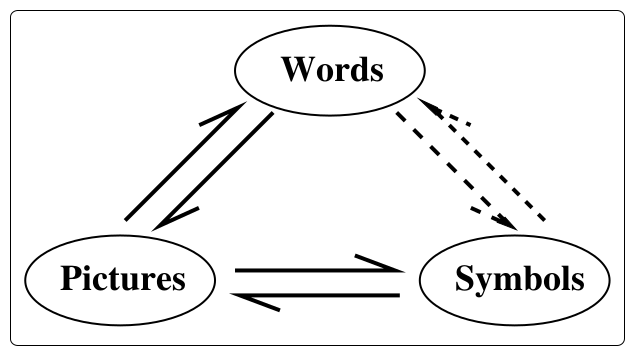
\includegraphics[scale=0.4]{imagens/palavras-imagens-simbolos.png}
    %
    %\footnotesize{Fonte:}
  \end{center}
\end{figure}

Professor Jerison's research focuses on PDEs and Fourier Analysis. He has taught single
variable calculus, multivariable calculus, and differential equations at MIT several
times each.

\paragraph{Professor Gigliola Staffilan}
Gigliola Staffilani is the Abby Rockefeller Mauzé Professor of Mathematics since 2007.
She received her Ph.D.\ from the University of Chicago in 1995. Following faculty
appointments at Stanford, Princeton, and Brown, she joined the MIT mathematics faculty
in 2002. She received both a teaching award and a research fellowship while at Stanford.
She received a Sloan Foundation Fellowship in 2000. In 2014 she was elected to the
American Academy of Arts and Sciences.

\begin{figure}[H]
  \begin{center}
    \caption{Professor Gigliola Staffilani}
    \label{fig:gigliola}
    \fbox{
\includegraphics[scale=0.7]{imagens/getting-started/staffilani.jpg}}
    %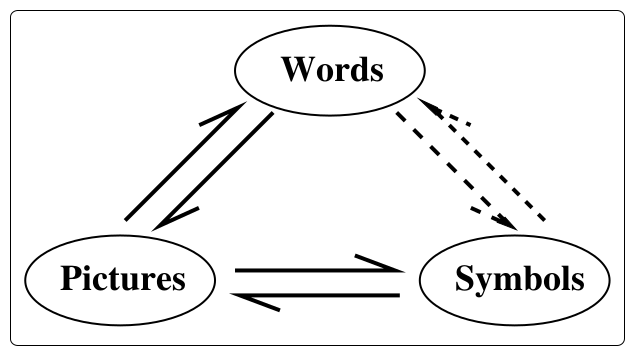
\includegraphics[scale=0.4]{imagens/palavras-imagens-simbolos.png}
    %
    %\footnotesize{Fonte:}
  \end{center}
\end{figure}

Professor Staffilani is an analyst, with a concentration on dispersive nonlinear PDEs.
She has taught multivariable calculus several times at MIT, as well as differential
equations.

\paragraph{Instructor Jen French}
Jen French is an MITx Digital Learning Scientist in the MIT math department. She earned
her Ph.D.\ in mathematics from MIT in 2010, with specialization in Algebraic Topology.
After teaching after school math for elementary aged students and working with the
Teaching and Learning Lab at MIT developing interdisciplinary curricular videos tying
foundational concepts in math and science to engineering design themes, she joined
MITx in 2013. She has developed videos, visual interactives, and problems providing
immediate feedback using the edX platform residentially in the MIT math department
to aid student learning. She has developed the calculus series (3 courses) and differential
equations series (5 courses) available here on edX.

\begin{figure}[H]
  \begin{center}
    \caption{Instructor Jen French }
    \label{fig:jen}
    \fbox{
\includegraphics[scale=0.7]{imagens/getting-started/french.jpg}}
    %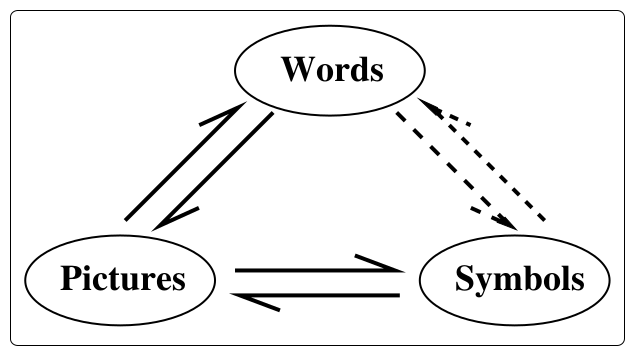
\includegraphics[scale=0.4]{imagens/palavras-imagens-simbolos.png}
    %
    %\footnotesize{Fonte:}
  \end{center}
\end{figure}

\paragraph{Instructor Karene Chu}
Karene Chu received her Ph.D.\ in mathematics from the University of Toronto in 2012.
Since then she has been a postdoctoral fellow first at the University of Toronto/Fields
Institute, and then at MIT, with research focus on knot theory. She has taught single
and multi-variable calculus, and linear algebra at the University of Toronto where
she received a teaching award.

\begin{figure}[H]
  \begin{center}
    \caption{Instructor Karene Chu}
    \label{fig:wang}
    \fbox{
\includegraphics[scale=0.7]{imagens/getting-started/karene.jpg}}
  \end{center}
\end{figure}

\paragraph{Special thanks to \ldots}
Professor Arthur Mattuck for starting it all.

Ed Tech Developers:
\begin{itemize}[noitemsep]
\item Phillip Ai
\item J.\ M.\ Claus
\item Eric Heubel
\item Haynes Miller
\item Martin Segado
\end{itemize}

MITx Video Team:
\begin{itemize}[noitemsep]
\item Brittany Bellamy
\item Chris Boebel
\item Tsinu Heramo
\item Douglass McLean
\item Lana Scott
\item Catilin Stier
\end{itemize}

\newpage
MITx Support Staff:
\begin{itemize}[noitemsep]
\item Kyle Boots
\item Brad K.\ Goodman
\end{itemize}

\fbox{\begin{minipage}{10cm}This course was funded in part by:\ \\
Class of 1960 Alumni Funds\ \\
2014--2015 Alumni Class Funds Grant\ \\
Wertheimer Fund\end{minipage}}

%%%%%%%%%%%%%%%%%%%%%%%%%%%%%%%%%%%%%%%%%%%%%%%%%%%%%%%%%%%%%%%%%%%%%%%%%%%%%%%%%
\subsubsection{Course description}
\label{gs-ol-description}

Discover the integral --- what it is and how to compute it. See how to use calculus
to model real world phenomena. Part 2 of 3.

How long should the handle of your spoon be so that your fingers do not burn while
mixing chocolate fondue? Can you find a shape that has finite volume, but infinite
surface area? How does the weight of the rider change the trajectory of a zip line
ride? These and many other questions can be answered by harnessing the power of the
integral. But what is an integral? You will learn to interpret it geometrically as
an area under a graph, and discover its connection to the derivative. You will encounter
functions that you cannot integrate without a computer and develop a big bag of tricks
to attack the functions that you can integrate by hand. The integral is vital in engineering
design, scientific analysis, probability and statistics. You will use integrals to find
centers of mass, the stress on a beam during construction, the power exerted by a motor,
and the distance traveled by a rocket.

This course, in combination with \emph{18.01.1x Calculus 1A: Differentiation}, covers the
AP Calculus AB curriculum.

This course, in combination with \emph{18.01.1x Calculus 1A: Differentiation} \textbf{and}
\emph{18.01.3x Calculus 1C: Coordinate Systems and Infinite Series}, covers the AP Calculus BC
curriculum.

If you intend to take an AP exam, we strongly suggest that you familiarize yourself with
the AP exam to prepare for it. 

%%%%%%%%%%%%%%%%%%%%%%%%%%%%%%%%%%%%%%%%%%%%%%%%%%%%%%%%%%%%%%%%%%%%%%%%%%%%%%%%%
\subsubsection{The making of this course}
\label{gs-ol-making}

This course was created using latex2edX, a free tool developed at MIT for creating
content for edX written in \LaTeX. \LaTeX\ is a typesetting language that is fantastic
for writing math! Occasionally, the equations you see in the webpage (which are rendered
in mathjax) do not load appropriately. Our apologies. The easiest fix is to simply
reload the page. Another solution is to change browsers. (Firefox seems to render
mathjax less reliably than Chrome or Safari. However, frequent changes to edX
will cause disruptions in our content.)

Note edX is not supported on tablet devices. That said, users report that 95\% of
the problems can be done on a tablet device, but if weird errors are creeping
in (especially with formula input type problems) you may try switching to a laptop
or desktop computer.

\begin{figure}[H]
  \begin{center}
    %\caption{}
    \label{fig:latex2edx}
    \fbox{
\includegraphics[scale=0.7]{imagens/getting-started/latex2edx.png}}
  \end{center}
\end{figure}
 
%%%%%%%%%%%%%%%%%%%%%%%%%%%%%%%%%%%%%%%%%%%%%%%%%%%%%%%%%%%%%%%%%%%%%%%%%%%%%%%%%
\subsubsection{How to succeed}
\label{gs-ol-succeed}

\paragraph{Prerequisites}
This course has a global audience with students from a wide variety of backgrounds.
To succeed in this course, you must have a solid foundation in

\begin{enumerate}[noitemsep]
\item Algebra
\item Geometry
\item Trigonometry
\item Exponents
\item Logarithms
\item Limits
\end{enumerate}

Because we know you come from different backgrounds, we want to help you to choose
the best path through this content. To aid us in this, please take the
``Choose your calculus adventure'' diagnostics. This will help you to determine
if you have the skills to succeed, what skills you may need to review, and which
units you may be able to skip!

\paragraph{Reference materials}
The material we provide in the Courseware contains all of the content you need for
this course. However, there are many good calculus texts that have a great deal of
problems and alternate explanations that may help you. Most widely used calculus
texts are adequate.

There is also the free web resource \href{https://www.khanacademy.org/}{Khan Academy}.
Links to other web resources can be found on the Course Info page under the header
``Related Links''. Feel free to share other resources on the course wiki or through
the discussion forum.

%%%%%%%%%%%%%%%%%%%%%%%%%%%%%%%%%%%%%%%%%%%%%%%%%%%%%%%%%%%%%%%%%%%%%%%%%%%%%%%%%
\subsubsection{Grading}
\label{gs-ol-grading}

There are 4 categories of graded problems in 18.01.2x: in-lecture Exercises,
Part A Homework, Part B Homework, and the Final Exam.

\begin{itemize}
\item \textbf{Exercises:} These are the problems that are interspersed between videos
  in each lecture. These problems count for 20\% of your grade. These problems will
  be used to motivate theory, practice a concept you just learned, and review material
  from previous sequences that we are using. While you are graded on these problems,
  they are low-stakes: you have multiple attempts, and have the opportunity to look
  at the answer after you have submitted a correct answer or run out of attempts.
  This is where you will do the majority of your learning. We encourage you to make
  mistakes and learn from them!
\item \textbf{Part A Homework:} Each unit has 1 Part A Homework assignment, which
  gives you an opportunity to practice what you learned. These problems count for 10\% o
  f your total grade. Wait until the end of the unit to attempt these problems.
  These problems help you identify the concepts that you have forgotten, and aid in
  long-term retention. These problems are mostly mechanical–asking you to practice
  methods, and techniques learned in each unit. Each problem typically tests knowledge
  from only one section in a unit. (We won't necessarily tell you which one though!)
\item \textbf{Part B Homework:} Each unit has 1 Part B Homework assignment. The part
  B homework counts for 25\% of your total grade. The problems on this homework
  combine ideas from all of the sequences in the unit. These problems are mostly in
  the form of word problems which ask you to apply the methods learned to new scenarios.
\item \textbf{Final:} The final exam is the culmination of your learning, and will
  account for 45\% of your grade. These problems cover all of the material in this course.
  Several of the problems follow the AP short-answer format. However, we cannot grade
  the justifications to your reasoning here. To prepare for the AP exam, you should
  take and review the solutions to sample AP exams from the AP website. 
\end{itemize}

\paragraph{Certification} To earn an ID verified certificate, you must earn 60\% of
the points in this course. You can see your progress towards certification by clicking
on the Progress link above.


%%%%%%%%%%%%%%%%%%%%%%%%%%%%%%%%%%%%%%%%%%%%%%%%%%%%%%%%%%%%%%%%%%%%%%%%%%%%%%%%%
%%%%%%%%%%%%%%%%%%%%%%%%%%%%%%%%%%%%%%%%%%%%%%%%%%%%%%%%%%%%%%%%%%%%%%%%%%%%%%%%%
\subsection{Using the EdX platform}
\label{gs-edx}

%%%%%%%%%%%%%%%%%%%%%%%%%%%%%%%%%%%%%%%%%%%%%%%%%%%%%%%%%%%%%%%%%%%%%%%%%%%%%%%%%
\subsubsection{Navigating EdX}
\label{gs-edx-nav}

This course was developed at MIT and is made available to you by the edX platform.
The edX platform is a platform for learning! It allows people from around the world
to access content for free, based on their own interests and background.

If you have never taken a course on edX, please take the short 1 hour course
\href{https://www.edx.org/course/demox-edx-demox-1-0}{DemoX} to familiarize yourself
with the platform and its capabilities.

In this course, we have the following top-level resources:

\begin{itemize}[noitemsep]
\item \textbf{Course:} This is the graded content of this course, as well as all
  learning materials.
\item \textbf{Calendar:} All of the due dates are in UTC, and are available in
  the google calendar, which you can download into your own calendar so that you
  can have these due dates available in your own time zone.
\item \textbf{Discussion:} This is a link to the full discussion forum. For
  specific discussions related to a problem or video, link through the discussion
  forum link at the bottom of each page. (See the discussion at the bottom of
  this page for help with these problems.)
\item \textbf{Progress:} Use this tab to see how your are progressing through
  the content!
\end{itemize}

\textbf{Course} is where you will spend most of your time. This is where we
put the content and assessments for your learning. Everything else is a resource
to support your learning.

%%%%%%%%%%%%%%%%%%%%%%%%%%%%%%%%%%%%%%%%%%%%%%%%%%%%%%%%%%%%%%%%%%%%%%%%%%%%%%%%%
\subsubsection{Example problem types}
\label{gs-edx-example}

Take a moment to familiarize yourself with the main problem types we use in this
course.

\textbf{Checking and submitting an answer:}

\begin{figure}[H]
  \begin{center}
    %\caption{}
    \label{fig:exqst01}
    \fbox{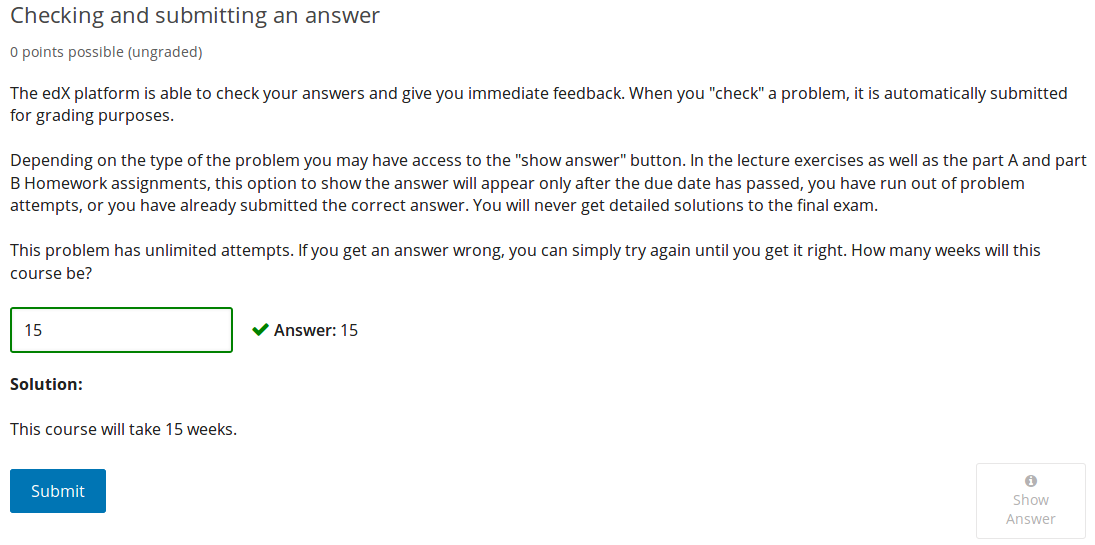
\includegraphics[scale=0.33]{imagens/getting-started/question-01.png}}
  \end{center}
\end{figure}

\textbf{Resetting a Problem:}

\begin{figure}[H]
  \begin{center}
    %\caption{}
    \label{fig:exqst02}
    \fbox{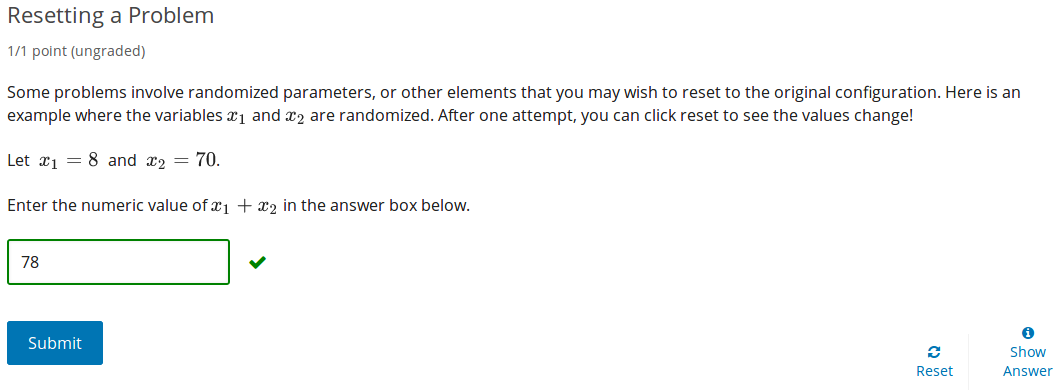
\includegraphics[scale=0.35]{imagens/getting-started/question-02.png}}
  \end{center}
\end{figure}

\newpage
\textbf{Limited Number of Attempts 1:}

\begin{figure}[H]
  \begin{center}
    %\caption{}
    \label{fig:exqst03}
    \fbox{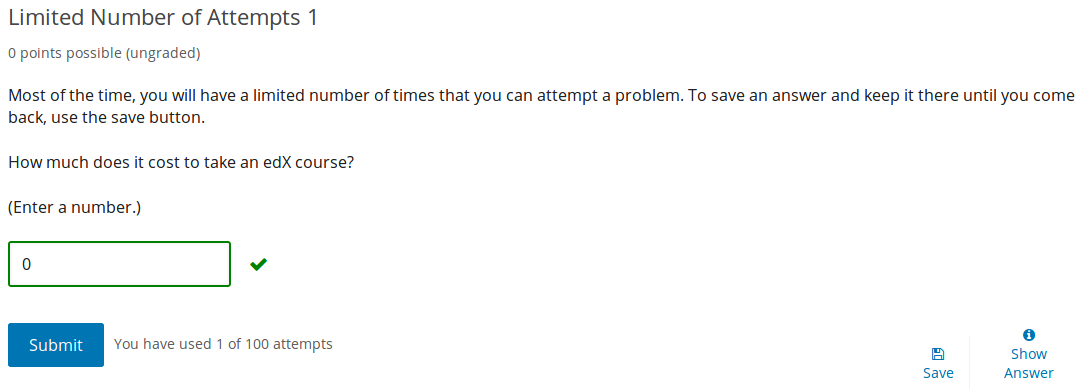
\includegraphics[scale=0.35]{imagens/getting-started/question-03.png}}
  \end{center}
\end{figure}

\textbf{Limited Number of Attempts 2:}

\begin{figure}[H]
  \begin{center}
    %\caption{}
    \label{fig:exqst04}
    \fbox{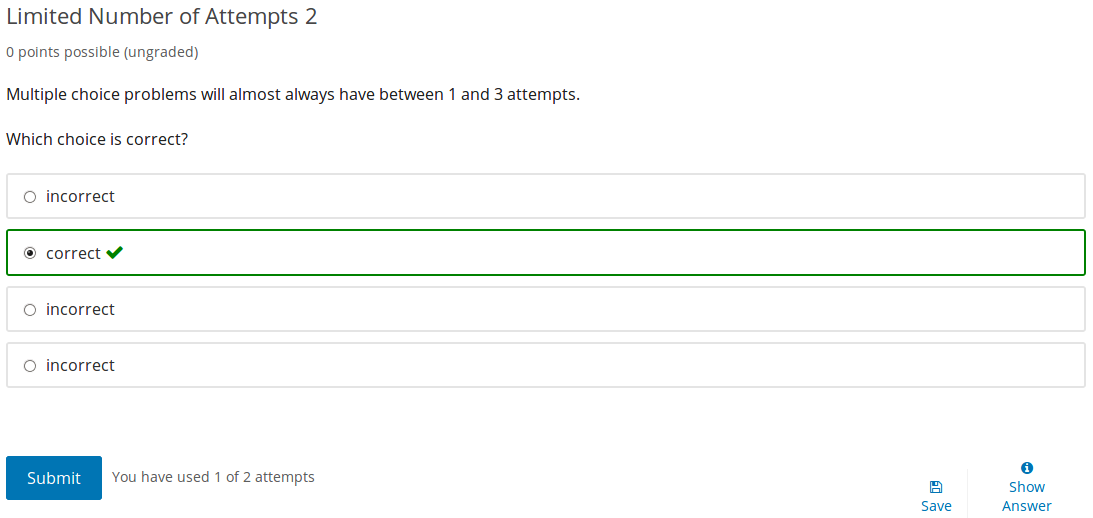
\includegraphics[scale=0.35]{imagens/getting-started/question-04.png}}
  \end{center}
\end{figure}

\textbf{Formula Entry Problems:}
This is a math class, which means we are going to be using formulas. And sometimes,
we want you to find these formulas. There are some rules for entering formulas into
the text entry box (which follows rules for ASCII math). Use:

\begin{itemize}[noitemsep]
\item Use $+$ to denote addition; e.g. $2+3$.
\item Use $-$ to denote subtraction; e.g. $x-1$.
\item Use $*$ to denote multiplication; e.g. $2*x$.
\item Use $\wedge$ to denote exponentiation; e.g. $x\wedge 2$ for $x^2$.
\item Use $/$ to denote division; e.g. 7$/$x for $7/x$.
\item Type \textbf{pi} for the mathematical constant $\pi$.
\item Type \textbf{e} for the mathematical constant $e$.
\item Type \textbf{sqrt(x)}, \textbf{sin(x)}, \textbf{cos(x)}, \textbf{ln(x)},
  \textbf{arccos(x)}, etc. for the known functions $\sqrt{x}$, $\sin{x}$, $\cos{x}$,
  $\ln{x}$, $\arccos{x}$, etc. Note that parentheses are required.
\item Use parentheses ( ) to specify order of operations.
\end{itemize}

Each formula entry box will have a Formula Input Help button below the answer button,
where you can find these facts about how to enter formulas. (See the button below.)

\begin{figure}[H]
  \begin{center}
    %\caption{}
    \label{fig:exqst05}
    \fbox{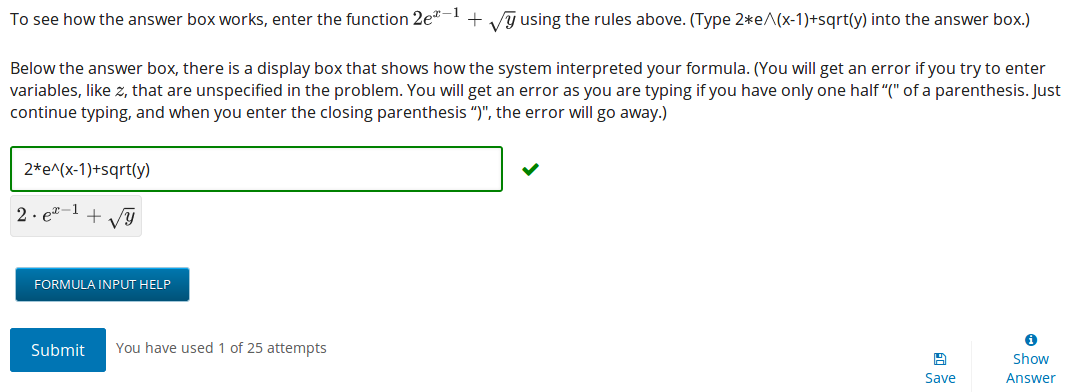
\includegraphics[scale=0.3]{imagens/getting-started/question-05.png}}
  \end{center}
\end{figure}

\textbf{Drag and Drop Problems:}

\begin{figure}[H]
  \begin{center}
    %\caption{}
    \label{fig:exqst06}
    \fbox{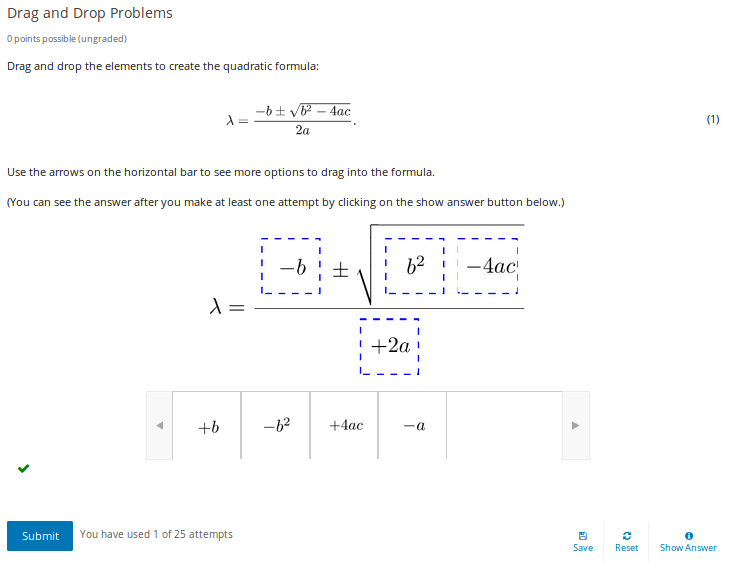
\includegraphics[scale=0.3]{imagens/getting-started/question-06.png}}
  \end{center}
\end{figure}

\textbf{Sketch Input Problems:}

\begin{figure}[H]
  \begin{center}
    %\caption{}
    \label{fig:exqst07}
    \fbox{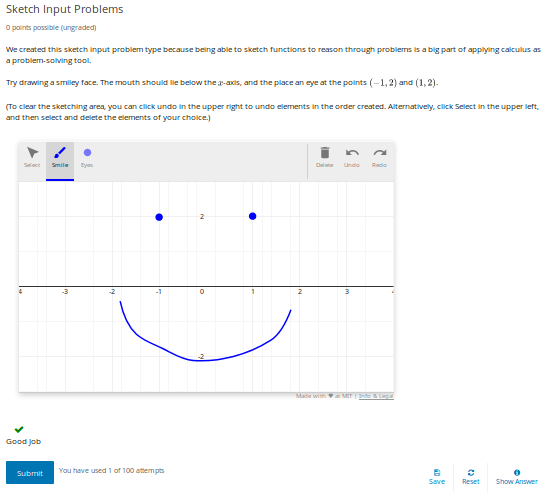
\includegraphics[scale=0.3]{imagens/getting-started/question-07.png}}
  \end{center}
\end{figure}

%%%%%%%%%%%%%%%%%%%%%%%%%%%%%%%%%%%%%%%%%%%%%%%%%%%%%%%%%%%%%%%%%%%%%%%%%%%%%%%%%
%%%%%%%%%%%%%%%%%%%%%%%%%%%%%%%%%%%%%%%%%%%%%%%%%%%%%%%%%%%%%%%%%%%%%%%%%%%%%%%%%
\subsection{Using the forum}
\label{gs-forum}

%%%%%%%%%%%%%%%%%%%%%%%%%%%%%%%%%%%%%%%%%%%%%%%%%%%%%%%%%%%%%%%%%%%%%%%%%%%%%%%%%
\subsubsection{Discussion forum}
\label{gs-forum-forum}

The discussion forum is the tool for connecting with the community of online learners
in this course. Use the forum to ask questions, seek clarifications, report bugs,
start or respond to topical discussions.

On most pages, there is a link at the bottom, which says ``show discussion''.
Clicking this link will show the discussion forum associated with the videos
and problems on that page.

\paragraph{``Netiquette'': What to do}

\begin{itemize}[noitemsep]
\item \textbf{Be polite.} Make sure that your posts are respectful of the other
  students and staff in the course.
\item Use the search button. Search for similar forum posts \textbf{before you
  post} using the magnifying glass icon. Many of your classmates will have the
  same question that you do! If you perform a search first, you may find the
  question and answer without needing to post yourself. This helps us keep the
  forum organized and useful!
\item Reply to existing discussions when you see someone with the same question.
  This helps to organize responses.
\item Use a descriptive and specific title to your post. This will attract the
  attention of TAs and classmates who can answer your question.
\item Be very specific about where you need help. Are you stuck on a particular
  part of a problem? Are you confused by a particular concept? What have you
  done so far?
\item Actively up-vote other posts, and other students will up-vote yours!
  The more up-votes your post has, the more likely they are to be seen.
\end{itemize}

\paragraph{``Netiquette'': What not to do}
Follow common writing practices for online communication:

\begin{itemize}[noitemsep]
\item Avoid TYPING IN ALL CAPS. Some people read this as shouting, even if
  that is not your intention.
\item Avoid \textbf{typing in bold}. Some people read this as shouting,
  even if that is not your intention.
\item Avoid unnecessary symbols, abbreviated words, texting shorthand,
  and replacing words with numbers (e.g. Pls don't rplce wrds w/\#s).
\item Avoid repeating letters or reeeeepeeaattinggggg chaaracterrrss.
\item Avoid excessive punctuation!!!!!!!!
\end{itemize}

\paragraph{Cheating!}
We encourage you to communicate in the forum about problems, and get hints
and help understanding the material from your fellow classmates and the
course TAs. However:

\begin{itemize}[noitemsep]
\item Please do not post solutions to lecture problems, homework
  problems (part A or part B), or final exam problems. These will be
  removed, and the student who posted will be contacted and dealt
  with individually.
\item Do not post or copy solutions posted to the forum for any exercises.
  This is cheating.
\item Do not copy solutions from yourself. This is cheating.
\end{itemize}


%%%%%%%%%%%%%%%%%%%%%%%%%%%%%%%%%%%%%%%%%%%%%%%%%%%%%%%%%%%%%%%%%%%%%%%%%%%%%%%%%
%%%%%%%%%%%%%%%%%%%%%%%%%%%%%%%%%%%%%%%%%%%%%%%%%%%%%%%%%%%%%%%%%%%%%%%%%%%%%%%%%
\subsection{Syllabus and schedule}
\label{gs-syllabus}

%%%%%%%%%%%%%%%%%%%%%%%%%%%%%%%%%%%%%%%%%%%%%%%%%%%%%%%%%%%%%%%%%%%%%%%%%%%%%%%%%
\subsubsection{Syllabus and schedule}
\label{gs-syllabus-syllabus}


%%%%%%%%%%%%%%%%%%%%%%%%%%%%%%%%%%%%%%%%%%%%%%%%%%%%%%%%%%%%%%%%%%%%%%%%%%%%%%%%%
%%%%%%%%%%%%%%%%%%%%%%%%%%%%%%%%%%%%%%%%%%%%%%%%%%%%%%%%%%%%%%%%%%%%%%%%%%%%%%%%%
\subsection{Getting to know you}
\label{gs-know}

%%%%%%%%%%%%%%%%%%%%%%%%%%%%%%%%%%%%%%%%%%%%%%%%%%%%%%%%%%%%%%%%%%%%%%%%%%%%%%%%%
\subsubsection{Getting to know you}
\label{gs-know-know}

%%%%%%%%%%%%%%%%%%%%%%%%%%%%%%%%%%%%%%%%%%%%%%%%%%%%%%%%%%%%%%%%%%%%%%%%%%%%%%%%%
\subsubsection{Prerequisite Knowledge}
\label{gs-know-pre}

%%%%%%%%%%%%%%%%%%%%%%%%%%%%%%%%%%%%%%%%%%%%%%%%%%%%%%%%%%%%%%%%%%%%%%%%%%%%%%%%%
\subsubsection{Integration diagnostics}
\label{gs-know-diag}


%%%%%%%%%%%%%%%%%%%%%%%%%%%%%%%%%%%%%%%%%%%%%%%%%%%%%%%%%%%%%%%%%%%%%%%%%%%%%%%%%
%%%%%%%%%%%%%%%%%%%%%%%%%%%%%%%%%%%%%%%%%%%%%%%%%%%%%%%%%%%%%%%%%%%%%%%%%%%%%%%%%
\subsection{Entrance Survey}
\label{gs-survey}

%%%%%%%%%%%%%%%%%%%%%%%%%%%%%%%%%%%%%%%%%%%%%%%%%%%%%%%%%%%%%%%%%%%%%%%%%%%%%%%%%
\subsubsection{Entrance Survey}
\label{gs-survey-survey}




%%%%%%%%%%%%%%%%%%%%%%%%%%%%%%%%%%%%%%%%%%%%%%%%%%%%%%%%%%%%%%%%%%%%%%%%%%%%%%%%%
%%%%%%%%%%%%%%%%%%%%%%%%%%%%%%%%%%%%%%%%%%%%%%%%%%%%%%%%%%%%%%%%%%%%%%%%%%%%%%%%%
%%%%%%%%%%%%%%%%%%%%%%%%%%%%%%%%%%%%%%%%%%%%%%%%%%%%%%%%%%%%%%%%%%%%%%%%%%%%%%%%%
\newpage
\section{Unit 1: The Integral}
\label{u1}


%%%%%%%%%%%%%%%%%%%%%%%%%%%%%%%%%%%%%%%%%%%%%%%%%%%%%%%%%%%%%%%%%%%%%%%%%%%%%%%%%
%%%%%%%%%%%%%%%%%%%%%%%%%%%%%%%%%%%%%%%%%%%%%%%%%%%%%%%%%%%%%%%%%%%%%%%%%%%%%%%%%
\subsection{Mean Value Theorem}
\label{u1-mvt}

%%%%%%%%%%%%%%%%%%%%%%%%%%%%%%%%%%%%%%%%%%%%%%%%%%%%%%%%%%%%%%%%%%%%%%%%%%%%%%%%%
\subsubsection{Motivation}
\label{u1-mvt-motiv}

Video: \href{https://www.youtube.com/watch?v=9B-XGTaHqXk}{Mean Value Theorem}

--- How you doing today, sir?

--- Hi.

--- Can I see your license and registration please?

--- What was I doing?

--- Speeding.

--- I was?

--- Yes, you were.

--- How do you know I was speeding?

--- You're looking a little tired. How long you've driving today?

--- Maybe two hours.

--- We did you come from?

--- New Jersey.

--- How far away is New Jersey?

--- 170 miles.

--- So 170 miles divided by 2 is 85 miles an hour, sir. Isn't that a little fast?

--- OK. So you knew my average speed was 85, but how do you know there was an incident
when I was traveling at 85?

--- Sir, it's simple math. The \emph{mean value theorem} states that one moment
your instantaneous speed is going to match your average speed.

\begin{figure}[H]
  \begin{center}
    %\caption{}
    \label{fig:mvt-motiv}
    \fbox{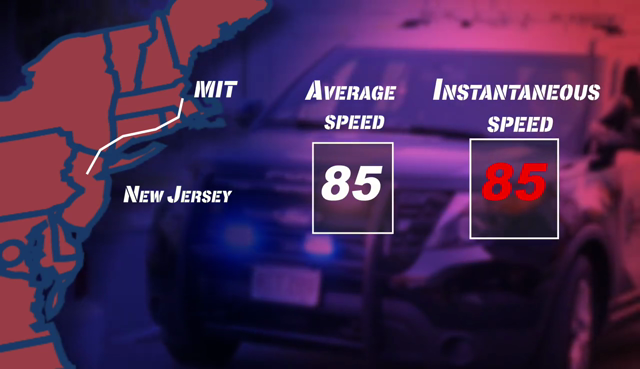
\includegraphics[scale=0.5]{imagens/unit-1/u1-m1-00001.png}}
  \end{center}
\end{figure}

--- You got me.

--- OK. Can I have that license and registration now, sir?

%%%%%%%%%%%%%%%%%%%%%%%%%%%%%%%%%%%%%%%%%%%%%%%%%%%%%%%%%%%%%%%%%%%%%%%%%%%%%%%%%
\subsubsection{The Mean Value Theorem and some applications}
\label{u1-mvt-applications}

Objectives:

\begin{itemize}[noitemsep]
\item Know the hypothesis and conclusion of the \textbf{Mean Value Theorem}
\item Use \textbf{upper bounds} and \textbf{lower bounds} on the derivative
  to establish inequalities between functions
\end{itemize}

Contents: 19 pages (9 videos, 33 minutes 1x speed, 35 questions)

%%%%%%%%%%%%%%%%%%%%%%%%%%%%%%%%%%%%%%%%%%%%%%%%%%%%%%%%%%%%%%%%%%%%%%%%%%%%%%%%%
\subsubsection{Exploration: Average vs instantaneous rate of change}
\label{u1-mvt-avgxinst}

\begin{Exercise}[title={Review of the average rate of change}]
  \noindent Recall the definition of the average rate of change of a function $x(t)$ over an
  interval $[a, b]$:
  \begin{equation}
    \text{Average Rate of Change} = \frac{x(b) - x(a)}{b - a}
  \end{equation}
  \noindent Geometrically, the average rate of change over $[a, b]$ is the slope of:
  \begin{itemize}[noitemsep]
  \bolota the secant line through $(a, x(a))$, $(b, x(b))$
  \bolota the tangent line through $(a, x(a))$
  \bolota the tangent line through $(b, x(b))$
  \end{itemize}
\end{Exercise}

\begin{Exercise}[title={Draw your answer, average rate of change}]
  \noindent Draw your answer from the previous problem on the graph below:
  \begin{figure}[H]
    \begin{center}
      %\caption{}
      \label{fig:mvt-avgxinst-2}
      \fbox{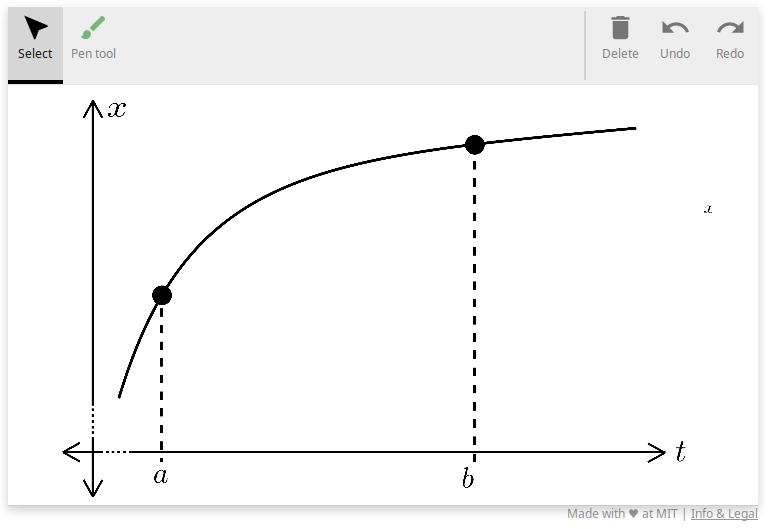
\includegraphics[scale=0.35]{imagens/unit-1/u1-m1-00002.png}}
    \end{center}
  \end{figure}
\end{Exercise}

\begin{Exercise}[title={Review of instantaneous rate of change}]
  \noindent Recall the instantaneous rate of the change of the function $x(t)$
  is the derivative: 
  \begin{equation}
    x'(t) = \lim_{\Delta t \to 0} \frac{x(t + \Delta t) - x(t)}{\Delta t}
  \end{equation}
  \noindent Geometrically, the instantaneous rate of change at $t$ is the slope of:
  \begin{itemize}[noitemsep]
  \bolota the secant line through $(t, x(t)$, $(b, x(b))$
  \bolota the tangent line through $(t, x(t))$
  \bolota the secamt line through $(a, x(a))$, $(t, x(t))$
  \end{itemize}
\end{Exercise}

\begin{Exercise}[title={Draw your answer, instantaneous rate of change}]
  \noindent Draw your answer from the previous problem on the graph below:
  \begin{figure}[H]
    \begin{center}
      %\caption{}
      \label{fig:mvt-avgxinst-3}
      \fbox{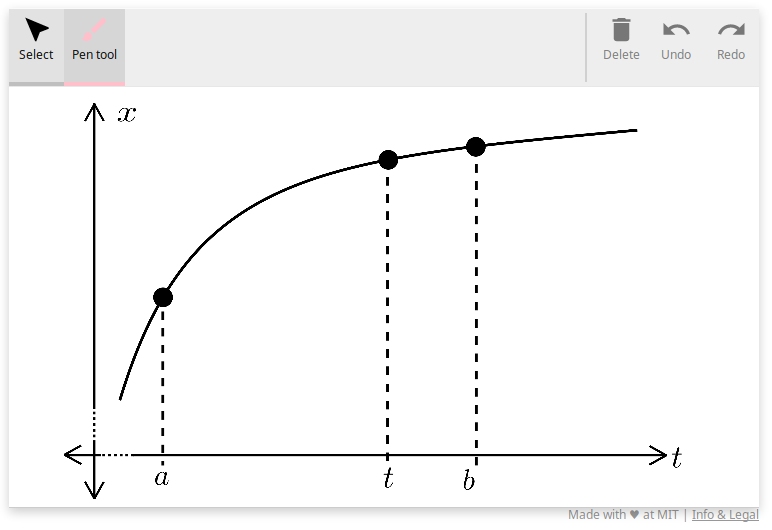
\includegraphics[scale=0.35]{imagens/unit-1/u1-m1-00003.png}}
    \end{center}
  \end{figure}
\end{Exercise}

\begin{Exercise}[title={Comparing average and instantaneous rates of change}]
  \noindent On the graph below, the secant line through $(a, x(a))$, $(b, x(b))$,
  has the same slope as the tangent line(s) at which of the following point(s)?
  (Check all that apply.)
  \begin{figure}[H]
    \begin{center}
      %\caption{}
      \label{fig:mvt-avgxinst-4}
      \fbox{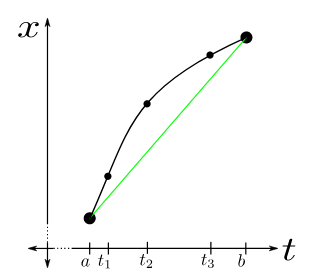
\includegraphics[scale=0.4]{imagens/unit-1/u1-m1-00004.png}}
    \end{center}
  \end{figure}
  \begin{itemize}[noitemsep]
    \quadrado $a$
    \quadrado $t1$
    \quadrado $t2$
    \quadrado $t3$
    \quadrado $b$
  \end{itemize}  
\end{Exercise}

Video: \href{https://www.youtube.com/watch?v=8yMIILYAxkw}{Mean Value Theorem: Conclusion}

The \emph{Mean Value Theorem (MVT)} relates the average rate of change
and the instantaneous rate of change of a function.
In more detail, consider a function
$x(t)$, over an interval $[a, b]$, so that the endpoints are
$(a, x(a))$ and $(b, x(b))$:

\begin{figure}[H]
  \begin{center}
    %\caption{}
    \label{fig:mvt-avgxinst-5}
    \fbox{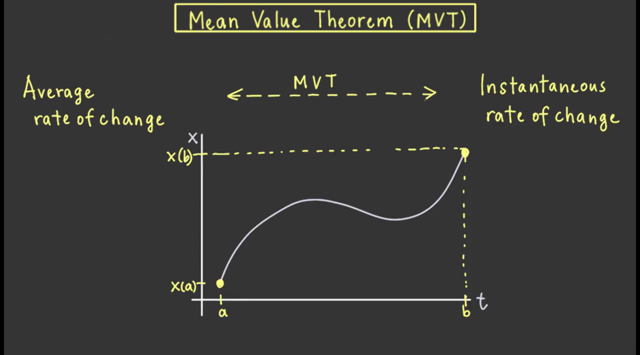
\includegraphics[scale=0.5]{imagens/unit-1/u1-m1-00005.png}}
  \end{center}
\end{figure}

Recall the average rate of change of the function
$x(t)$ over the interval $[a, b]$ is geometrically
the slope of the secant line through the two endpoints:

\begin{figure}[H]
  \begin{center}
    %\caption{}
    \label{fig:mvt-avgxinst-6}
    \fbox{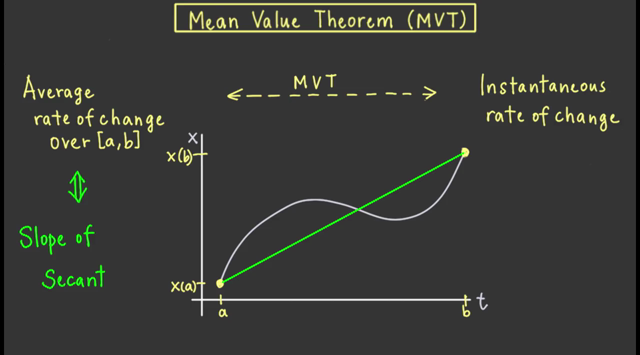
\includegraphics[scale=0.5]{imagens/unit-1/u1-m1-00006.png}}
  \end{center}
\end{figure}

Recall also that the instantaneous rate
of change of the function $x(t)$,
at a point $t_1$ between $a$ and $b$, is geometrically
the slope of the tangent line at $t_1$:

\begin{figure}[H]
  \begin{center}
    %\caption{}
    \label{fig:mvt-avgxinst-7}
    \fbox{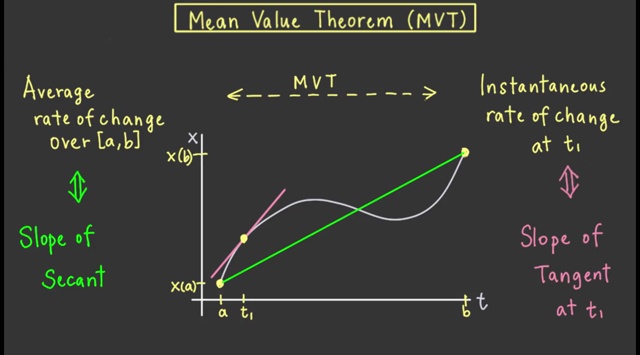
\includegraphics[scale=0.5]{imagens/unit-1/u1-m1-00007.png}}
  \end{center}
\end{figure}

Notice the average rate of change is only one number,
but the instantaneous rate of change
can take different values at different points
within the interval:

\begin{figure}[H]
  \begin{center}
    %\caption{}
    \label{fig:mvt-avgxinst-8}
    \fbox{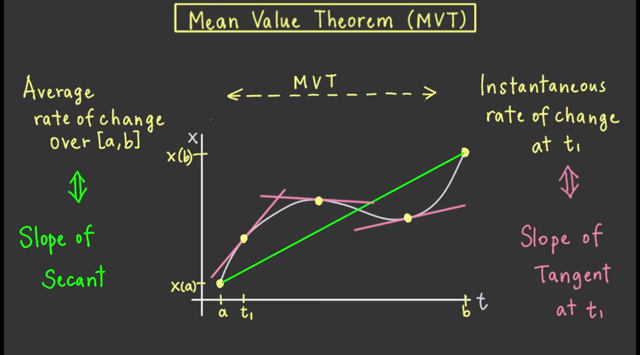
\includegraphics[scale=0.5]{imagens/unit-1/u1-m1-00008.png}}
  \end{center}
\end{figure}

So how does the mean value theorem relate to these two?
Well, as you will see on our graph,
there is a point at which the tangent
is parallel, in other words, has the same slope
as the secant line.

Let us find such a point now.
We can shift the secant line without changing its slope
until it is tangent to our graph.
And here it is at a point at which the tangent is parallel
to the secant.
And we will call this point $c$:

\begin{figure}[H]
  \begin{center}
    %\caption{}
    \label{fig:mvt-avgxinst-9}
    \fbox{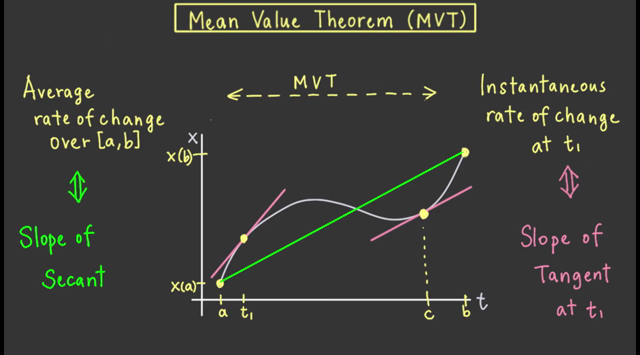
\includegraphics[scale=0.5]{imagens/unit-1/u1-m1-00009.png}}
  \end{center}
\end{figure}

So the following is the conclusion
of the mean value theorem:
\textbf{there is some point $c$, in between the endpoints $a$
and $b$, such that the average rate of change from $a$ to $b$
is equal to the instantaneous rate of change at $c$}:

\begin{figure}[H]
  \begin{center}
    %\caption{}
    \label{fig:mvt-avgxinst-10}
    \fbox{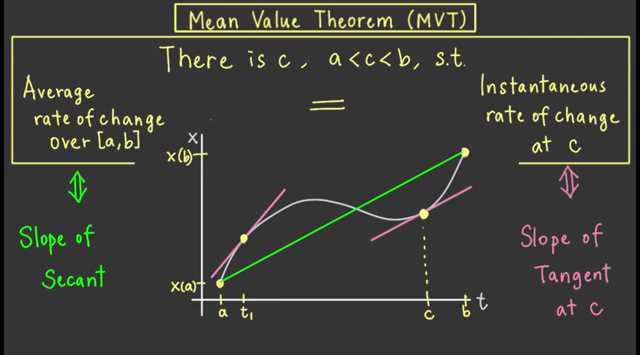
\includegraphics[scale=0.5]{imagens/unit-1/u1-m1-00010.png}}
  \end{center}
\end{figure}

Or again, geometrically, \textbf{there is some point $c$, in between $a$
and $b$, such that the slope of the secant line through the two
endpoints is equal to the slope of the tangent line at $c$}.

Notice the MVT says that such a $c$ is \emph{strictly
in between the endpoints}, but it does not
say where exactly such a $c$ is, or even
\emph{how many} such $c$'s there are.
In fact, there are two such $c$'s in our example:

\begin{figure}[H]
  \begin{center}
    %\caption{}
    \label{fig:mvt-avgxinst-11}
    \fbox{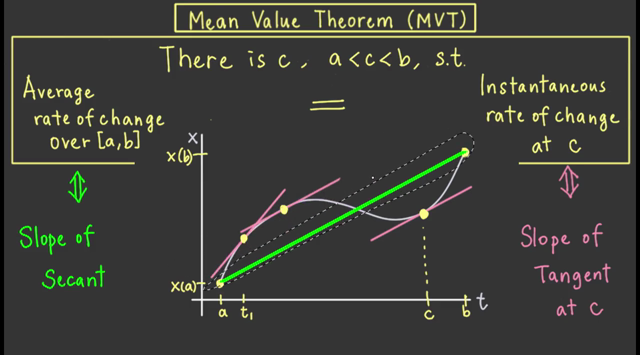
\includegraphics[scale=0.5]{imagens/unit-1/u1-m1-00011.png}}
  \end{center}
\end{figure}

We have only talked about the conclusion of the mean value
theorem. But what about the hypothesis?
In other words, \emph{when does it hold}?
To find out when the theorem holds,
let us now explore \emph{when it fails}.

%%%%%%%%%%%%%%%%%%%%%%%%%%%%%%%%%%%%%%%%%%%%%%%%%%%%%%%%%%%%%%%%%%%%%%%%%%%%%%%%%
\subsubsection{Identifying necessary hypotheses}
\label{u1-mvt-hypot}

\begin{Exercise}[title={How the Mean Value Theorem can go wrong}]
  \noindent The MVT conclusion: \textbf{There is a point $c$, such that $a<c<b$, at
    which the tangent line is parallel to the secant line through $(a, x(a))$ and
    $(b, x(b))$}. We may abbreviate ``such that'' with ``s.t.'' from now on.
  For which of the graphs below is the MVT conclusion false? (Solid points are
  the end points. Dotted lines are asymptotes. Check all that apply.) 
  \begin{figure}[H]
    \begin{center}
      %\caption{}
      \label{fig:mvt-hypot-1}
      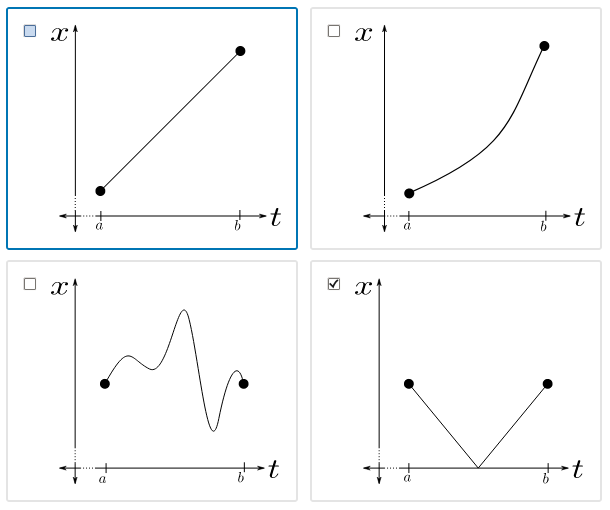
\includegraphics[scale=0.4]{imagens/unit-1/u1-m1-00012.png}
    \end{center}
  \end{figure}
  \begin{figure}[H]
    \begin{center}
      %\caption{}
      \label{fig:mvt-hypot-2}
      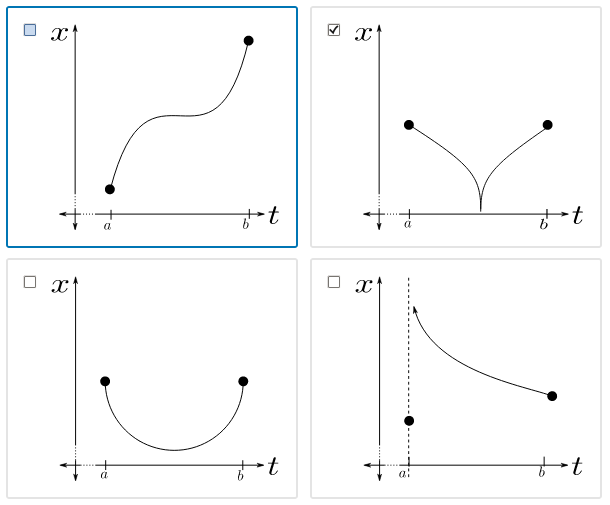
\includegraphics[scale=0.4]{imagens/unit-1/u1-m1-00013.png}
    \end{center}
  \end{figure}
  \begin{figure}[H]
    \begin{center}
      %\caption{}
      \label{fig:mvt-hypot-3}
      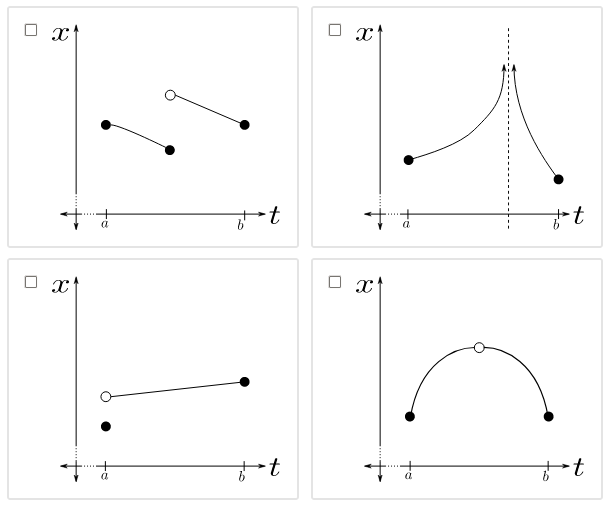
\includegraphics[scale=0.4]{imagens/unit-1/u1-m1-00014.png}
    \end{center}
  \end{figure}
\end{Exercise}

Video: \href{https://www.youtube.com/watch?v=WmAcRkkoqOA}{Mean Value Theorem: Full statement}

Here is the conclusion of the mean value theorem
that we have already seen: 
\textbf{There is some point $c$, between $a$ and $b$, at which the tangent is
parallel to the secant}. You have just seen that this statement
holds for some functions, but doesn't for some others.
So \emph{what are conditions that will guarantee
that the MVT conclusion holds}?

Let us investigate the examples from the problem you just
solved.
We have collected the successful functions,
the ones for which the MVT conclusion hold,
on the top row, and the failures,
on the bottom two rows:

\begin{figure}[H]
  \begin{center}
    %\caption{}
    \label{fig:mvt-hypot-4}
    \fbox{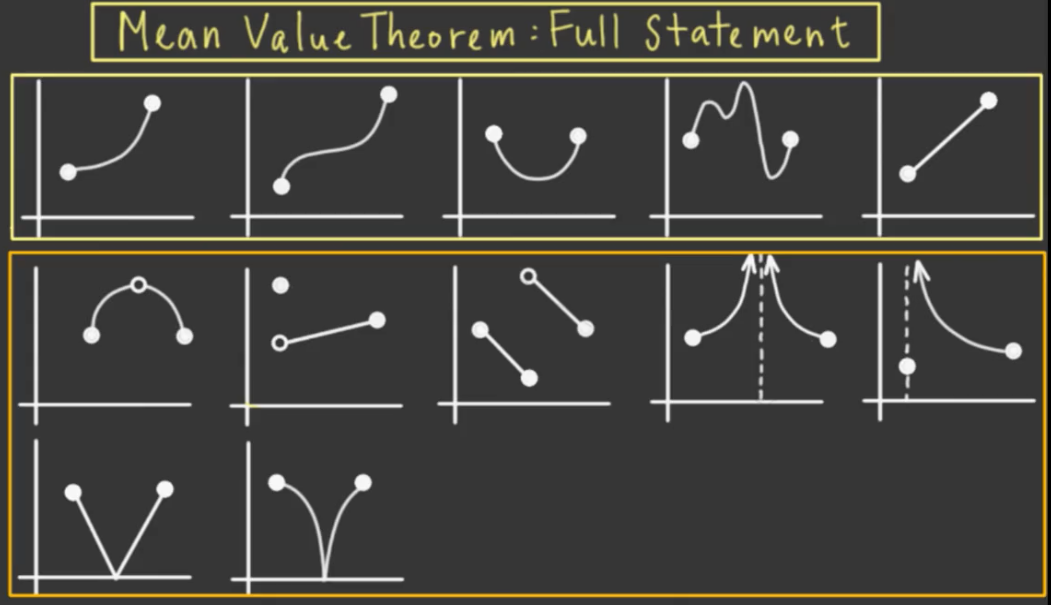
\includegraphics[scale=0.3]{imagens/unit-1/u1-m1-00015.png}}
  \end{center}
\end{figure}

We will start by discussing why the functions in the middle row
fail.
Let us look at the first graph.
For the first graph, we can shift the secant line
to approach a point where it is tangent to our graph.
But we find that the exact point that this would have happened
is a point where the function is undefined.
So there is no $c$:

\begin{figure}[H]
  \begin{center}
    %\caption{}
    \label{fig:mvt-hypot-5}
    \fbox{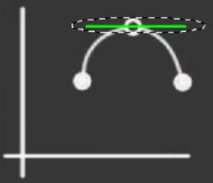
\includegraphics[scale=0.5]{imagens/unit-1/u1-m1-00016.png}}
  \end{center}
\end{figure}

Next, let's look at the second graph in the middle row.
It has a jump discontinuity at an endpoint.
The secant line slants down, but all the tangent lines slant up,
so there is no $c$.
Because of the discontinuity, there
is no relationship between the slope of the secant
and the slope of the tangents:

\begin{figure}[H]
  \begin{center}
    %\caption{}
    \label{fig:mvt-hypot-6}
    \fbox{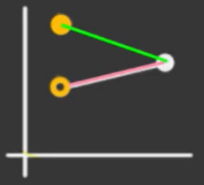
\includegraphics[scale=0.5]{imagens/unit-1/u1-m1-00017.png}}
  \end{center}
\end{figure}

Similarly, for the rest of the graphs in this row,
the reason that the MVT conclusion fails
is a discontinuity either at an endpoint
or within the interval:

\begin{figure}[H]
  \begin{center}
    %\caption{}
    \label{fig:mvt-hypot-7}
    \fbox{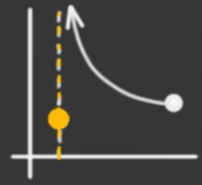
\includegraphics[scale=0.5]{imagens/unit-1/u1-m1-00018.png}}\\
    \fbox{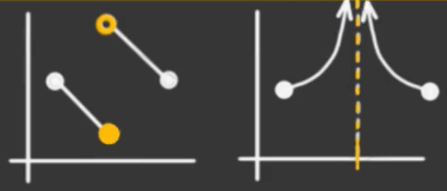
\includegraphics[scale=0.5]{imagens/unit-1/u1-m1-00019.png}}
  \end{center}
\end{figure}

Let's look at the bottom row now.
Each of these two graphs is continuous
but has a point within the interval where
the derivative does not exist.
In the first, there is a corner, and in the second,
there is a cusp:

\begin{figure}[H]
  \begin{center}
    %\caption{}
    \label{fig:mvt-hypot-8}
    \fbox{
\includegraphics[scale=0.5]{imagens/unit-1/u1-m1-00020.png}}
  \end{center}
\end{figure}

You can check that the reason there
is no tangent parallel to the secant
is because of the point where the function is not
differentiable.

Let us now look at the successful functions.
We can use the same method as before
to find a point at which the tangent is parallel
to the secant:

\begin{figure}[H]
  \begin{center}
    %\caption{}
    \label{fig:mvt-hypot-9}
    \fbox{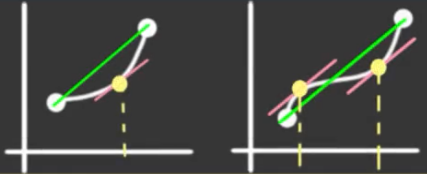
\includegraphics[scale=0.5]{imagens/unit-1/u1-m1-00021.png}}\\
    \fbox{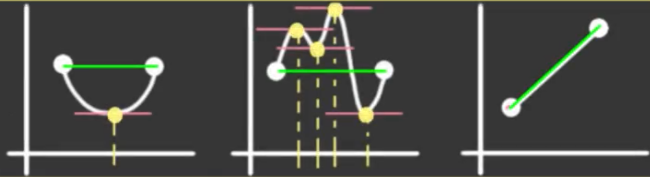
\includegraphics[scale=0.5]{imagens/unit-1/u1-m1-00022.png}}
  \end{center}
\end{figure}

We see that the first four graphs on this row
have hump shapes at whose peaks the $c$'s appear.
On the other hand, the last function on this row
is equal to the secant line, so at every point,
the tangent is also equal to the secant line.
In other words, every point within the interval is a $c$.

What do all these graphs have in common?
Well, all of these graphs are \emph{continuous and differentiable}.
Let's return to our question, what condition on a function
will guarantee that the MVT conclusion holds?
We already see that continuity and differentiability
are conditions that will include all
of our examples of successes, and exclude
all of our cases of failures.
It turns out that \emph{continuity and differentiability are
  enough to guarantee success}.

So let us state the mean value theorem precisely:
\textbf{If a function $x(t)$ is \emph{continuous}
on the closed interval $[a, b]$, and
\emph{differentiable} on the open interval $(a, b)$,
then there is some point $c$ in the open interval
$(a, b)$ such that the average rate of change from $[a, b]$
is equal to the instantaneous rate of change at $c$}:

\begin{figure}[H]
  \begin{center}
    %\caption{}
    \label{fig:mvt-hypot-10}
    \fbox{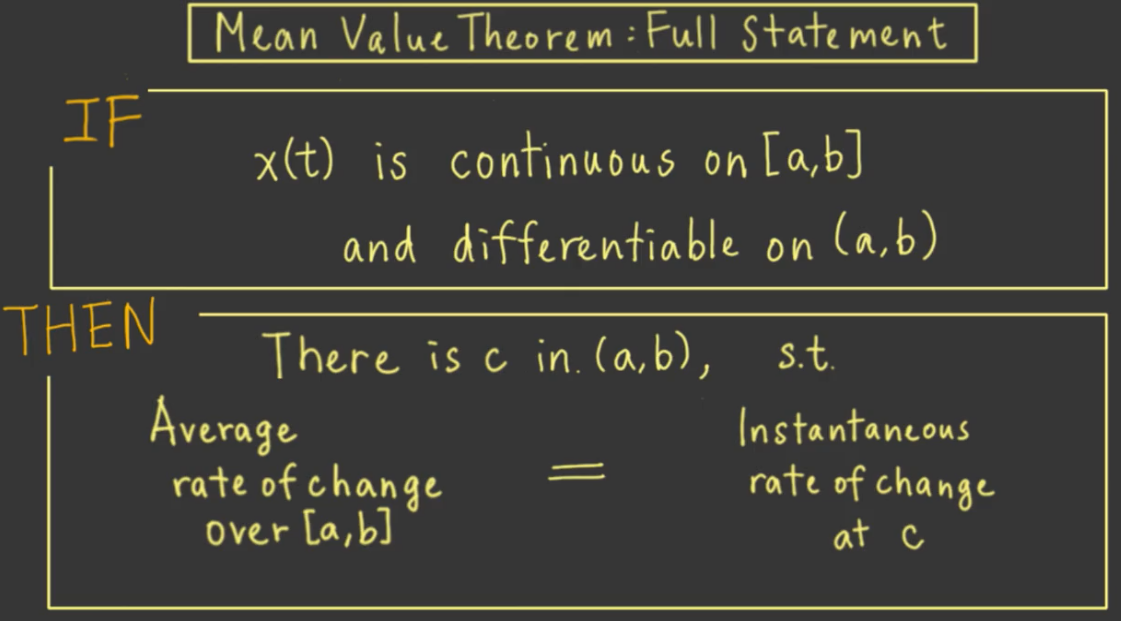
\includegraphics[scale=0.3]{imagens/unit-1/u1-m1-00023.png}}
  \end{center}
\end{figure}

Let's write this conclusion in terms of formulas
now rather than words:

\begin{equation}
  \frac{x(b) - x(a)}{b - a} = x'(c)
\end{equation}

Notice in the hypothesis the function:

\begin{itemize}[noitemsep]
\item needs to be continuous on the closed interval, including
  the endpoints;
\item needs to be differentiable only on the open interval (so the
  derivative does not have to exist for the endpoints)
\end{itemize}

Let us now do some exercises.
And we will continue with some immediate consequences
of the MVT.

%%%%%%%%%%%%%%%%%%%%%%%%%%%%%%%%%%%%%%%%%%%%%%%%%%%%%%%%%%%%%%%%%%%%%%%%%%%%%%%%%
\subsubsection{Statement of the Mean Value Theorem}
\label{u1-mvt-statement}

If $x(t)$ is continuous on $a \le t \le b$, and differentiable on $a < t < b$, that
is, $x(t)$ is defined for all $t$, $a < t < b$, then for some $c$ with $a < c < b$:

\begin{equation}
  \frac{x(b) - x(a)}{b - a} = x'(c)
\end{equation}

Equivalently, in geometric terms, there is at least one point $c$, with $a < c < b$,
at which the tangent line is parallel to the secant line through $(a, x(a))$ and
$(b, x(b))$:

\begin{figure}[H]
  \begin{center}
    %\caption{}
    \label{fig:mvt-stat-1}
    \fbox{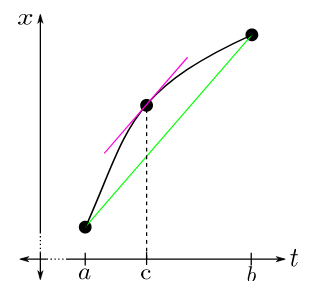
\includegraphics[scale=1]{imagens/unit-1/u1-m1-00024.png}}
  \end{center}
\end{figure}

\begin{Exercise}[title={The logic of the MVT}]
  \noindent The following graph has a discontinuity within the interval $[a, b]$:
  \begin{figure}[H]
    \begin{center}
      %\caption{}
      \label{fig:mvt-stat-2}
      \fbox{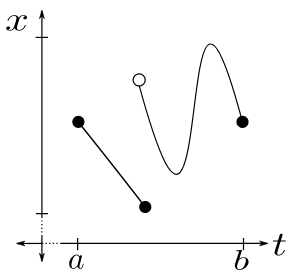
\includegraphics[scale=0.5]{imagens/unit-1/u1-m1-00025.png}}
    \end{center}
  \end{figure}
  \noindent Is there a point $c$ with $a < c < b$ at which the tangent line is
  parallel to the secant line through $(a, x(a))$ and $(b, x(b))$?
  \begin{itemize}[noitemsep]
    \bolota Yes
    \bolota No
  \end{itemize}
  \noindent What does this say about the MVT?
  \begin{itemize}[noitemsep]
    \bolota There can be no $c$ because the hypothesis of the MVT is not satisfied.
    \bolota This graph does not satisfy the MVT hypothesis but satisfies the MVT
    conclusion. This example does not contradict the MVT.
    \bolota This graph shows that the MVT statement above must have the wrong hypothesis.
    \bolota This graph shows that the MVT statement above must have the wrong conclusion.
  \end{itemize}
\end{Exercise}

\paragraph{Proof of the MVT:} To prove the Mean Value Theorem, we will start by proving
a special case in which the function has the same values at the two end points,
and then use this special case to prove the full theorem.

To prove the special case, we will rely on the \emph{Extreme Value Theorem}, which says
that any function which is continuous on a closed interval must attain both its
maximum and minimum values in that closed interval. This theorem requires deeper analysis
of the real numbers and we will not prove it here. The point is that we need continuity
to guarantee that the function attains both its maximum and minimum.

\textbf{Proof of the special case:}

Suppose a function $x_0(t)$ satisfies the hypothesis of the MVT, that is,
$x_0(t)$is continuous on $[a, b]$, and differentiable on $(a, b)$.

In this special case, suppose also that $x_0(a) = x_0(b)$. By the Extreme Value Theorem,
$x_0(t)$ attains both its maximum and minimum in $[a, b]$. In other words, there is at
least one point $t_1$ in $[a, b]$ such that $\displaystyle x_0(t_1) = \min_{a \le t \le b}x_0(t)$,
and at least one point $t_2$ in $[a, b]$ such that $\displaystyle x_0(t_2) = \max_{a \le t \le b}x_0(t)$.

There are only two possibilities. The maximum and minimum are either equal or not.

\begin{itemize}
\item Case 1: $\displaystyle \max_{a \le t \le b}x_0(t) = \min_{a \le t \le b}x_0(t)$\\
  In this case $x_0(t)$ must be constant over $[a, b]$, so $x'_0(t) = 0$ for all
  $a < t < b$. In particular, there is at least one point $c$, with $a < c < b$ at
  which $x'_0(c) = 0$. 
\item Case 2: $\displaystyle \max_{a \le t \le b}x_0(t) \ne \min_{a \le t \le b}x_0(t)$\\
  In this case, since $x_0(a) = x_0(b)$, they cannot be both at the end points.
  Hence at least one of $\displaystyle \max_{a \le t \le b}x_0(t)$ and $\displaystyle \min_{a \le t \le b}x_0(t)$
  must be achieved in $(a, b)$. Hence, there must be a $c$, with $a < c < b$ such that
  $\displaystyle x_0(c) = \max_{a \le t \le b}x_0(t)$ or $\displaystyle x_0(c) = \min_{a \le t \le b}x_0(t)$.
  Now, recall the derivative of a differentiable function at a local maximum or minimum.
  By the hypothesis, $x_0(t)$ is differentiable in $(a, b)$, so $x'_0(c) = 0$ since
  $c$ is either a local maximum or a minimum.
\end{itemize}

In both cases, since $x_0(a) = x_0(b)$, there is a point $c$, with $a < c < b$, such that
\begin{equation}
  x'_0(c) = 0 = \frac{0}{b-a} = \frac{x_0(b) - x_0(a)}{b-a}
\end{equation}

This special case of the MVT is called \textbf{Rolle's Theorem}.

Let us now use the special case above to prove the MVT for functions with possibly
different endpoint values.

Suppose a function $x(t)$
satisfies the hypothesis of the MVT, that is, $x(t)$ is continuous on $[a, b]$,
and differentiable on $(a, b)$. Let

\begin{equation}
  x_0(t) = x(t) - \left(x(a) + \frac{x(b) - x(a)}{b-a}(t-a)\right)
\end{equation}

That is, construct a function $x_0(t)$ by subtracting from $x(t)$ the line that goes through
$(a, x(a))$, $(b, x(b))$. Then $x_0(t)$ also satisfies the hypothesis of the MVT, and
$x_0(a) = x_0(b) = 0$. So we can apply Rolle's Theorem to $x_0(t)$, and know that there is a $c$
in $(a, b)$, such that $x'_0(c) = 0$.

Now we can rearrange the equation above and get $x(t)$ in terms of $x_0(t)$:

\begin{equation}
  x(t) = x_0(t) + \left(x(a) + \frac{x(b) - x(a)}{b-a}(t-a)\right)
\end{equation}

Taking the derivative on both sides. we get

\begin{equation}
  x'(t) = x'_0(t) + \frac{x(b) - x(a)}{b-a}
\end{equation}

And at the point $c$ in $(a, b)$ at which $x'_0(c) = 0$, the equation above reduces to

\begin{equation}
  \begin{split}
    x'(x) &= x'_0(c) + \frac{x(b) - x(a)}{b-a}\\
          &= \frac{x(b) - x(a)}{b-a}
  \end{split}
\end{equation}

Thus, we have found a $c$ we need for the conclusion of the MVT.

%%%%%%%%%%%%%%%%%%%%%%%%%%%%%%%%%%%%%%%%%%%%%%%%%%%%%%%%%%%%%%%%%%%%%%%%%%%%%%%%%
\subsubsection{Back to the speeding ticket example}
\label{u1-mvt-speed}

\begin{Exercise}[title={Time-position graph of the speeding car}]
  \noindent Recall in the example of the speeding car, the only information the
  police had was that our car was at the $50$ mile marker at $8$ a.m., and $220$
  mile marker at $10$ a.m. Let $x(t)$ be the position of the car at time $t$
  and let the units of $x$ be miles and $t$ be hours, so that $x(8) = 50$, and
  $x(10) = 200$. Which of the following graphs can be the graph of $x(t)$? Check all that applies.
  \begin{figure}[H]
    \begin{center}
      %\caption{}
      \label{fig:mvt-speed-1}
      \fbox{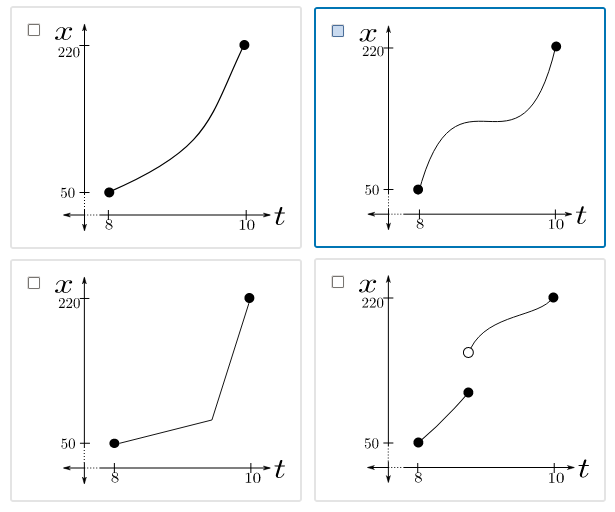
\includegraphics[scale=0.65]{imagens/unit-1/u1-m1-00026.png}}
    \end{center}
  \end{figure}
\end{Exercise}

\begin{Exercise}[title={When 85 mph?}]
  \noindent Recall the average velocity of the car between $8$ and $10$ am is $85$ mph.
  According to the MVT, the strongest conclusion the police officer could make about when
  the car is traveling at exactly $85$ mph is:

  \noindent ``There is/are (a)\_\_\_\_\_\_\_\_\_\_\_\_\_\_\_ such moment(s) (b)\_\_\_\_\_\_\_\_\_\_\_\_\_\_\_
  and he (c)\_\_\_\_\_\_\_\_\_\_\_\_\_\_\_ when such moment(s) is(are).''

  \noindent The (a) is:
  \begin{itemize}[noitemsep]
    \bolota no
    \bolota at least one
    \bolota exactly one
    \bolota more than one
  \end{itemize}

  \noindent The (b) is:
  \begin{itemize}[noitemsep]
    \bolota after 8, and before 10
    \bolota at or after 8, and before 10
    \bolota at 8 or at 10
  \end{itemize}

  \noindent The (c) is:
  \begin{itemize}[noitemsep]
    \bolota knows
    \bolota does not know
  \end{itemize}
\end{Exercise}

%%%%%%%%%%%%%%%%%%%%%%%%%%%%%%%%%%%%%%%%%%%%%%%%%%%%%%%%%%%%%%%%%%%%%%%%%%%%%%%%%
\subsubsection{Application to simultaneous rates}
\label{u1-mvt-speed}













%%%%%%%%%%%%%%%%%%%%%%%%%%%%%%%%%%%%%%%%%%%%%%%%%%%%%%%%%%%%%%%%%%%%%%%%%%%%%%%%%
%%%%%%%%%%%%%%%%%%%%%%%%%%%%%%%%%%%%%%%%%%%%%%%%%%%%%%%%%%%%%%%%%%%%%%%%%%%%%%%%%
%%%%%%%%%%%%%%%%%%%%%%%%%%%%%%%%%%%%%%%%%%%%%%%%%%%%%%%%%%%%%%%%%%%%%%%%%%%%%%%%%
%%%%%%%%%%%%%%%%%%%%%%%%%%%%%%%%%%%%%%%%%%%%%%%%%%%%%%%%%%%%%%%%%%%%%%%%%%%%%%%%%
%%%%%%%%%%%%%%%%%%%%%%%%%%%%%% TERMINA O DOCUMENTO %%%%%%%%%%%%%%%%%%%%%%%%%%%%%%
%%%%%%%%%%%%%%%%%%%%%%%%%%%%%%%%%%%%%%%%%%%%%%%%%%%%%%%%%%%%%%%%%%%%%%%%%%%%%%%%%
%%%%%%%%%%%%%%%%%%%%%%%%%%%%%%%%%%%%%%%%%%%%%%%%%%%%%%%%%%%%%%%%%%%%%%%%%%%%%%%%%
%%%%%%%%%%%%%%%%%%%%%%%%%%%%%%%%%%%%%%%%%%%%%%%%%%%%%%%%%%%%%%%%%%%%%%%%%%%%%%%%%
%%%%%%%%%%%%%%%%%%%%%%%%%%%%%%%%%%%%%%%%%%%%%%%%%%%%%%%%%%%%%%%%%%%%%%%%%%%%%%%%%
\end{document}
